\documentclass[9pt,twocolumn,twoside]{gsajnl}
% Use the documentclass option 'lineno' to view line numbers
\usepackage{booktabs}
\usepackage{siunitx}
\usepackage{adjustbox}
\usepackage{geometry} % just not to bother with the table width
%\usepackage[colorinlistoftodos]{todonotes} % comments in margins
%\setlength{\marginparwidth}{1.25cm}
%\definecolor{flame}{rgb}{0.89, 0.35, 0.13}
%\newcommand{\josh}[1]{\textcolor{flame}{\emph{\scriptsize {#1}}}}
%\newcommand{\citex}{\textcolor{red}{\bf (CITE)\,}}
%\newcommand{\out}[1]{\textcolor{red}{#1}} %outline placeholder text
\newcommand{\X}{\textcolor{red}{\bf X\,}}

\articletype{gos} % article type
% {inv} Investigation
% {gs} Genomic Selection
% {goi} Genetics of Immunity
% {gos} Genetics of Sex
% {mp} Multiparental Populations

\title{Reduced Nucleotide Diversity on a Plant Y Chromosome Following Recent Recombination Suppression}

\author[$\ast$,$\dagger$,1]{Josh Hough}
\author[$\dagger$]{Wei Wang}
\author[$\dagger$]{Spencer C.H. Barrett}
\author[$\dagger$]{Stephen I. Wright}

\affil[$\ast$]{Department of Plant Sciences, University of California, Davis}
\affil[$\dagger$]{Department of Ecology and Evolutionary Biology, University of Toronto}

%\affil[$\dagger$]{Author two affiliation}
%\affil[$\ddagger$]{Author three affiliation}
%\affil[$\S$]{Author four affiliation}
%\affil[$\ast\ast$]{Author five affiliation}

\keywords{Sex Chromosome Evolution; Nucleotide Diversity; Recombination; Deleterious Mutations}

\runningtitle{Plant sex chromosome evolution} % For use in the footer

\correspondingauthor{Josh Hough}

\begin{abstract}
X and Y chromosomes differ in effective population size ($N_{e}$), rates of recombination, and exposure to natural selection, all of which can significantly affect levels of genetic variability within the genome. On Y chromosomes with suppressed recombination, selection can remove genetically-linked neutral variation, resulting in reduced $N_{e}$ and the level of polymorphism on Y compared to X chromosomes or autosomes. However, non-selective factors including female biased sex ratios and high variance in male reproductive success can also reduce Y-linked $N_{e}$, making it difficult to infer the causes of low Y-chromosome diversity. Here, we investigate the factors affecting X- and Y-linked polymorphism during the early stages of plant sex chromosome evolution in \textit{Rumex hastatulus} (Polygonaceae). Strikingly, we find that nucleotide diversity on the Y is more than 40-fold lower than on the X, suggesting an extensive reduction in diversity. We demonstrate that the magnitude of diversity loss is inconsistent with a purely neutral model that accounts for the occurrence of female-biased sex ratios in this species, or by reduced male $N_{e}$ caused by high variance in male fitness. Rather, using forward simulations and population genetic estimates of the distribution of fitness effects of deleterious mutations, we show that Y diversity levels can be explained by the action of linked selection against deleterious mutations, although selective sweeps may also be playing a role. Given the recent origin of \textit{R. hastatulus} sex chromosomes, our study is consistent with the prediction that the early stages of Y chromosome degeneration are characterized by strong effects of selective interference experienced by a large number of selected sites, rather than simply neutral drift following gene silencing. 
\end{abstract}


\setboolean{displaycopyright}{true}

\begin{document}

\maketitle
\thispagestyle{firststyle}
\marginmark
\firstpagefootnote
\correspondingauthoraffiliation{jhough@ucdavis.edu}
\vspace{-11pt}

\section*{Introduction}

\lettrine[lines=2]{\color{color2}M}{}orphologically distinct sex chromosomes have evolved multiple times independently in both plant and animal kingdoms \citep{westergaard1958,ohno1967,bull1983,charlesworth1991}. Despite numerous biological differences between the kingdoms, X and Y chromosomes in both lineages have undergone similar genetic changes, suggesting that general evolutionary mechanisms might drive sex chromosome divergence \citep{charlesworth1978,charlesworth1996CB,charlesworth2000degeneration}. Investigating the shared features of plant and animal sex chromosomes, including the loss of recombination \citep{bergero2009}, the degeneration of Y chromosomes \citep{hough2014,bergero2015}, and the evolution of dosage compensation \citep{muyle2012,papadopulos2015}, thus provides an informative context for investigating the evolutionary forces driving sex chromosome evolution.

One fundamental difference between sex chromosomes and autosomes is their copy number in a population; whereas autosomes in diploid species are present in two copies in each sex, the X chromosome is present in two copies in females and only one copy in males. As a consequence, the effective population size ($N_{e}$) of the X chromosome is predicted to be 3/4 that of autosomes, whereas the $N_{e}$ of the male-limited Y chromosome is expected to equal 1/4 that of autosomes (assuming an equal number of reproducing females and males). Such differences in $N_{e}$ are predicted to directly affect relative levels of neutral polymorphism maintained on these chromosomes, which is proportional to the product of $N_{e}$ and the neutral mutation rate, $\mu$ \citep{Kimura1984}. Such variation in neutral polymorphism within the genome can have important consequences on patterns of DNA sequence evolution, including the effectiveness of both positive and negative selection \citep{charlesworth1987}.

Several demographic factors are expected to modulate or accentuate differences in neutral polymorphism maintained on sex chromosomes \citep{ellegren2009}. These include population subdivision and sex-biased dispersal, deviations from a 1:1 breeding sex ratio, and high sex-specific variance in reproductive success \citep{caballero1995,charlesworth2001,laporte2002,pool2007}. In theory, these processes all result in asymmetries in female vs male $N_{e}$, that could lead to different levels of neutral polymorphism on the sex chromosomes than are expected based on the autosomes (\citep{pool2007}). As evidence for this, coalescent simulations have shown that models of male-biased migration during human out-of-Africa dispersal result in levels of X/A neutral diversity similar to what is observed \citep{keinan2009} (though it is worth noting that there is considerable variation in current estimates of X/A in humans, and other demographic scenarios have been suggested \citep{hammer2010,bustamante2009}). In addition, disproportionate losses of sex-linked compared to autosomal variation arising from population bottleneck events have been inferred in chimpanzees and orangutans \citep{kaessmann2001,fischer2006}, the house mouse \textit{Mus musculus} \citep{baines2007}, and Drosophila \citep{andolfatto2001}, highlighting the importance of demography in affecting patterns of sex-linked and autosomal neutral variation.

In addition to demographic factors, evolutionary theory predicts that neutral variability on Y chromosomes with suppressed recombination can be significantly reduced by Hill-Robertson Interference (HRI), which causes a reduction in $N_{e}$ of neutral sites that are genetically linked to sites experiencing selection. The major types of HRI include (i) selection on strongly beneficial mutations ("selective sweeps") \citep{smith1974hitch,aquadro1994} (ii) selection against strongly deleterious mutations
) \citep{charlesworth1996background,charlesworth1994effect} \citep{charlesworth1996CB,charlesworth2000degeneration}, and (iii) intereference between weakly selected sites (weak selection Hill-Robertson interference). In all of these processes, linkage  disequilibrium between selected and neutral sites results in a level of neutral variation below the level predicted in the absence of selection. 


Consistent with an important role for Hill-Robertson interference in driving down diversity on the Y chromosome, studies examining Y chromosome variability in mammals \citep{hellborg2004,bachtrog2013NRG,Wilsonsayres2014} and Drosophila \citep{mcallister1999,bachtrog2000} have revealed that Y-linked diversity is considerably lower than predicted under models of neutral evolution, with linked selection playing a key role.


%discussion point?:
%Moreover, because recombination suppression was relatively recent on plant Y chromosomes, it is an open question whether weak-HRI has had enough time to have a large effect. Although selective interference (indlucing BGS and Selective Sweeps) is expected to have the greatest effects during the early stages of Y-chromosome evolution \citep{bachtrog2008temporal} the R. hastatulus Y chromosome has undergone significant degeneration and gene loss over a short period of time, suggesting that it may behave more similarly to more ancient Y chromosomes.


Despite widespread interest in determining the effects of recombination on patterns of genetic diversity \citep{ellegren2011,bachtrog2013NRG}, we still know very little about the influence of linked selection on patterns nucleotide polymorphism in younger sex chromosome systems, where \textit{de novo} recombination suppression evolved relatively recently \citep{charlesworth2016plant}. Background selection and selective sweeps are predicted to have the strongest effects during the earliest stages of Y-chromosome evolution, before Y-chromosomes have lost the majority of their genes. On the other hand, if gene silencing and Y inactivation occur very early during the process of Y chromosome degeneration, it is possible that the strength of linked selection is minimal even on relatively young Y chromosomes, and that much degeneration may occur neutrally following the silencing of Y-linked genes. 

To investigate the factors affecting nucleotide diversity in the early stages of sex chromosome evolution, we analyzed single nucleotide polymorphisms (SNPs) on sex chromosomes and autosomes in the plant \textit{R. hastatulus }(Polygonaceae). This species is a dioecious annual with highly heteromorphic X and Y chromosomes that are estimated to have evolved  approximately 15 MYA \citep{quesada2011,grabowska2015,navajas2005}, making sex chromosomes in this species over 100 million years younger than the well-studied mammalian sex chromosomes \citep{lahn1999,ross2005dna}. \textit{Rumex hastatulus} has also received particular attention because of the unique occurrence of an intraspecific sex chromosome system, in which both XY and $XY_{1}XY_{2}$ males occur in geographically distinct 'chromosomal races' \citep{smith1963mechanism}. The $XY_{1}XY_{2}$ sex chromosome system in this species (the North Carolina race) is thought to have originated through an X-autosome fusion, with the XY system (the Texas race) maintaining the ancestral chromosome complement \citep{smith1964evolving}. Despite the recent origin of sex chromosomes in both races, a recent study revealed that both the ancestral and neo-Y chromosomes have undergone significant gene loss and functional deterioration \citep{hough2014}.

Of particular relevance to the present study, \textit{R. hastatulus} populations have also been found to consistently exhibit female-biased sex ratios, with a mean sex ratio of $N_{m}/N_{f}=0.6$ \citep{pickup2013influence}. This is important because female-biased sex ratios are predicted to affect chromosomal $N_{e}$ and therefore the level of neutral polymorphism maintained on sex chromosomes and autosomes \citep{ellegren2009}. Here, we test whether patterns of nucleotide diversity on sex chromosomes and autosomes in \textit{R. hastatulus} are jointly consistent with neutral evolutionary processes - including the effects of sex ratio bias and variance in reproductive success - or whether the removal of linked neutral variation caused by positive and purifying selection has played a more significant role.

\section*{Materials and Methods}
\subsection*{Population Samples and Sex-Linked Genes}
We analyzed sex-linked and autosomal genes identified from Illumina RNA sequence data from 24 individuals (12 males and 12 females, with 1 male and 1 female from each of 12 populations; 6 populations of each sex chromosome race). Samples were collected in 2010 from throughout the native range of \textit{R. hastatulus} (locations in Table S1), and plants were grown in the glasshouse from seeds collected from open-pollinated females. We extracted RNA from leaf tissue using Spectrum Plant Total RNA kits (Sigma-Aldrich). The isolation of mRNA and cDNA synthesis was conducted according to standard Illumina RNAseq procedures, with sequencing conducted on two Illumina HiSeq lanes with 150-bp end reads at the Genome Quebec Innovation Center. Reads from these 24 samples were mapped to the \textit{R. hastatulus} reference transcriptome \citep{hough2014}, and raw sequences are available from the Gen-Bank Short Read Archive under accession no. SRP041588. Reads were mapped using the Burrows–Wheeler Aligner \citep{li2010fast}, followed by Stampy \citep{lunter2011stampy}. We used Picard tools (http://picard.sourceforge.net) to modify mapping output into the format required for the Genome Analysis Toolkit \citep{mckenna2010genome} variant calling software, and subsequently removed genes with low coverage (<10x) and Phred Quality Scores <20. The population samples analyzed here were previously reported in Hough et al. (2014), where they were used to validate the ascertainment of sex-linked genes identified through segregation analysis. Here, to consider sex linked genes that were identified in each of our sequenced population samples, we focused on the set of 460 X/Y genes for which the Y homolog was found in both the Texas and North Carolina races (i.e., X/Y genes where the Y copy was inferred to be on the $Y_{1}$ chromosome).

\subsection*{Autosomal Genes}
In evaluating evidence for nucleotide diversity differences between X and Y chromosomes, it is important to distinguish between reduced Y-linked diversity, and the possibility that X-linked diversity is elevated above the level predicted from a neutral model. To do this, we normalized sex-linked diversity estimates by autosomal diversity, and compared empirical X/A and Y/A nucleotide diversity ratios to those predicted from neutral models and from simulations (described below). Because the criteria for identifying autosomal loci in Hough et al. (2014) were based on the occurrence of four segregating SNPs per locus, this set of genes is probably higher in diversity than the average autosome. Therefore, for the present analysis we incorporated the broader set of all non-sex linked (putatively autosomal) genes from our transcriptome data. We also filtered this set to remove genes that may have been sex-linked but were not identified as such by Hough et al.'s conservative ascertainment criteria. In particular, we removed: (i) any genes in which there was evidence for at least one SNP with a sex-linked segregation pattern, (ii) any genes with SNPs showing fixed heterozygosity in males and fixed homozygosity in females, (iii) any genes with less than 10X coverage or greater than 100X coverage from independently obtained genomic coverage data (to filter out duplicate genes or those with highly repetitive sequences), and (iv) any genes containing SNPs with large (>0.4) allele frequency differences between males and females. Finally, we removed genes with fewer than 100 synonymous sites following this filtering to avoid biasing our results toward genes that may have been particularly short due to assembly problems. This filtering resulted in a set of 12,356 and 11,350 autosomal genes in the Texas and North Carolina races, respectively.

\subsection*{Phasing X and Y alleles}
To estimate polymorphism for the X and Y sequences separately, it is necessary to infer the phase of SNPs in sex-linked transcripts in males. In previous work, phasing alleles on \textit{R. hastatulus} sex chromosomes was achieved using segregation analysis from a genetic cross. Here, to phase SNPs from population samples where such segregation data was unavailable, we used HAPCUT \citep{bansal2008hapcut}, a maximum-cut based algorithm that reconstructs haplotypes using sequenced fragments (Illumina read data) from the two homologous chromosomes to output a list of phased haplotype blocks containing the SNP variants on each chromosome. Because the resulting haplotype blocks produced by HAPCUT contained SNPs that were phased relative to each other, but not designated to either the X or Y chromosome, we assigned individual variants to X or Y by independently identifying fixed X-Y differences with each haplotype block (i.e., sites in which all females were homozygous, and all males were heterozygous). Identifying such fixed differences within phased haplotype blocks enabled us to then infer the correct phase (X or Y) of the polymorphisms from HAPCUT’s output. This was done by matching the phase of fixed X-Y differences with their neighboring polymorphic sites: when a fixed X-Y difference occurred in the same phased haplotype block as a polymorphic site, the polymorphic variants in that block were assigned to either X or Y based on the known phase of the fixed difference with which they were matched. SNPs that were identified outside of phased blocks, or in blocks without fixed X-Y differences, were recorded as missing data. Finally, we filtered out SNPs with coverage > 60, QUAL score > 60, and those within a distance of 10bp or less from indels. This procedure was conducted using a combination of Perl and Bash scripts, and resulted in fasta-formatted alignments of X and Y sequences for 372 sex-linked genes from the 24 individuals in our study.

We further validated the results of HAPCUT’s allele phasing by comparing the accuracy of this method with the phasing-by-segregation method that was conducted in Hough et al. (2014). To do this, we first phased the sequence data from parents and their progeny using HAPCUT’s algorithm (using the same parameters as for the population data), and then identified cases where SNPs were inferred on the Y chromosome by HAPCUT, but where the ‘true’ level polymorphism was known to be zero. We identified 7 percent of sex-linked genes with phasing errors of this kind, or which were otherwise determined to have genotyping errors resulting in false SNP calls. This corresponds to a SNP error rate estimate of 1.7 x 10-4. Note that this rate is very low relative to population-based estimates of polymorphism on the X and autosomes (Table 1), and therefore should have minimal effects on our estimation of X/A polymorphism. However, because the rate is high relative to the expected level of true polymorphism on the Y-chromosome, we  further filtered genes in which we found evidence for false-positive Y-polymorphisms arising from: (i) phasing errors caused by gene duplicates (more than two haplotypes), (ii) polymorphisms around indels, and (iii) genotyping errors caused by low Y-expression. This filtering was done by manually inspecting sequences in IGV \citep{robinson2011integrative} and identifying each individual putative polymorphism on the Y chromosome.

\subsection*{Estimating nucleotide diversity on sex chromosomes and autosomes}
For each locus in our analysis, we calculated Watterson’s (1975) estimator of the population parameter $\theta=4N_{e}\mu$, where $N_{e}$ is the effective population size, and $\mu$ is the mutation rate \citep{watterson1975}, using a modified version of the Perl program Polymorphurama \citep{bachtrog2006}. To compare sex-linked and autosomal loci, we calculated the average value of $\theta$, weighted by the number of synonymous sites in each gene (\X Figure 2; Table 1). We obtained 95 percent confidence intervals for our estimates of the X/A and Y/A diversity ratios by bootstrapping by gene using the BCa method \citep{efron1994} implemented in the Boot package in R \citep{canty2012boot}, and calculating X/A and Y/A diversity on each iteration for 20000 replicates each. Bootstrapping was conducted on the final filtered set of 173 sex-linked, and 12355 autosomal genes from the Texas race, and separately for the 176 sex-linked and 11349 autosomal genes from the North Carolina race. Note that the lack of recombination on the Y chromosome implies that assumptions about independence across loci are likely violated, suggesting that the true uncertainty in our Y/A diversity estimate may be wider than implied by bootstrapping across genes. To address this issue, we also used a maximum likelihood approach, implemented in a modified version of the MLHKA software \citep{wright2004hka} to independently estimate a credibility interval for the Y/A ratio (Figure S1). Because of the thousands of genes involved, a likelihood method incorporating divergence to control for heterogeneity in mutation rate is not feasible, since this would involve maximizing the likelihood estimate of the mutation rate for each locus independently.  Therefore, we applied a method that assumed no heterogeneity in mutation rate, no recombination between Y-linked genes, and free recombination between autosomal loci. Our model therefore had two parameters; theta for autosomal genes and the Y/A ratio. We varied both parameters across a grid of points and evaluated the likelihood, where the Y/A ratio varied from 0.001 to 1, and Watterson's theta on the autosomes varied from 0.001 to 0.01. We also tested whether estimates of diversity for the X chromosome calculated from phased sequences from females were consistent with estimates from phased sequences from males. As no significant difference was observed (\X Figure? Table?), we report only results from females.

Finally, we tested for population substructure within and between the two sex chromosome races to control for the possibility that hidden substructure in our sampled populations could affect estimates of diversity. To do this, we constructed neighbor-joining trees of sex-linked sequences from all populations in our study. The analysis was conducted on an alignment of the X- and Y-linked genes from \textit{R. hastatulus}, with orthologous autosomal sequences from the non-dioecious but closely related outgroup species \textit{R. bucephalophorus} used to root the tree (Figure S2). We used the Neighbor-Joining method \citep{saitou1987neighbor}, with evolutionary distances computed using Maximum Composite Likelihood \citep{tamura2011mega5}. The inferred trees revealed strong support for Y-linked genes from the $XY_{1}XY_{2}$ ("North Carolina") race being paraphyletic (98\% bootstrap support), with samples from two populations (hereafter the "SC sub-clade") forming a monophyletic group, and samples from Florida and Georgia (hereafter the "FL sub-clade") also forming a monophyletic group, that was more closely related to the XY ("Texas") race (Figure S2). In light of this evidence for significant population substructure, and to consider between-population differences, we estimated X and Y diversity in each of the three sub-clades (SC, FL, TX) separately.

\subsection*{Neutral predictions and the effect of sex ratio bias on diversity}
To test whether the levels of diversity we observed on X, Y and autosomal chromosomes could be explained by the occurrence of biased reproductive sex ratios or high variance in reproductive success, we compared our empirical diversity estimates to predictions from a neutral model that jointly considers these two effects. Here, following Nomura (2002), the neutrally-expected effective population size for autosomal loci is given by:

\begin{equation}
N_{e{A}} = \frac{4N_{m}N_{f}}{N_{m}(1+C^2_{f})+N_{f}(1+C^2_{m})}\label{eq:NeA}
\end{equation}

where $N_{m}$ and $N_{f}$ are effective population sizes for males and females, respectively, and $C^2_{i}$ is the coefficient of variation in mating success for the $i$th sex, defined as the ratio of the standard deviation to the mean number of mates $\sigma_{i}/\mu_{d{i}}$. Similarly, for X and Y linked loci,

\begin{equation}
N_{e{X}} = \frac{9N_{m}N_{f}}{4N_{m}(1+C^2_{f})+2N_{f}(1+C^2_{m})}\label{eq:NeX}
\end{equation}

and

\begin{equation}
N_{e{Y}} = \frac{N_{m}(1+C^2_{f})}{2}\label{eq:NeY}
\end{equation}

With no variation in mating success in either sex ($C^2_{m}=C^2_{f}=0$), equations 1-3 reduce to the familiar expressions from \citep{wright1931evolution}:

\begin{equation}
N_{e{A}} = \frac{4N_{m}N_{f}}{N_{m}+N_{f}}\label{eq:NeA}
\end{equation}


\begin{equation}
N_{e{X}} = \frac{9N_{m}N_{f}}{4N_{m}+2N_{f}}\label{eq:NeX}
\end{equation}

\begin{equation}
N_{e{Y}} = \frac{N_{m}}{2}\label{eq:NeY}
\end{equation}

To consider the joint effects of biased sex ratios and variance in male reproductive success, neutrally-expected levels of diversity were calculated using equations 1-3, assuming no variance in female mating (e.g., $C^2_{f}=0$), and we considered a range of values for $\sigma_{m}$: 0 (no variance), 1/2 (Poisson/2) 1 (Poisson distribution of offspring), 2 (Poisson*2), and 3 (Poisson*3). Figure 1 shows the predicted effective population size of autosomes and sex chromosomes as a function of the sex ratio under this model. Using these predictions, we calculated the expected X/A and Y/A ratios of diversity for the estimated \textit{R. hastatulus} sex ratio $N_{m}/N_{f}=0.6$ \citep{pickup2013influence}, assuming that the level of neutral polymorphism is given by the product of the mutation rate and the effective population size, $\theta=4N_{e}\mu$ \citep{watterson1975}. Note that we considered variance in male reproductive success here because this is most likely to occur in wind pollinated plant like \textit{R. hastatulus}, where males produce copious amounts of pollen and compete to fertilize uniovulate female flowers (\X ref).

\begin{figure}[htbp]
\centering
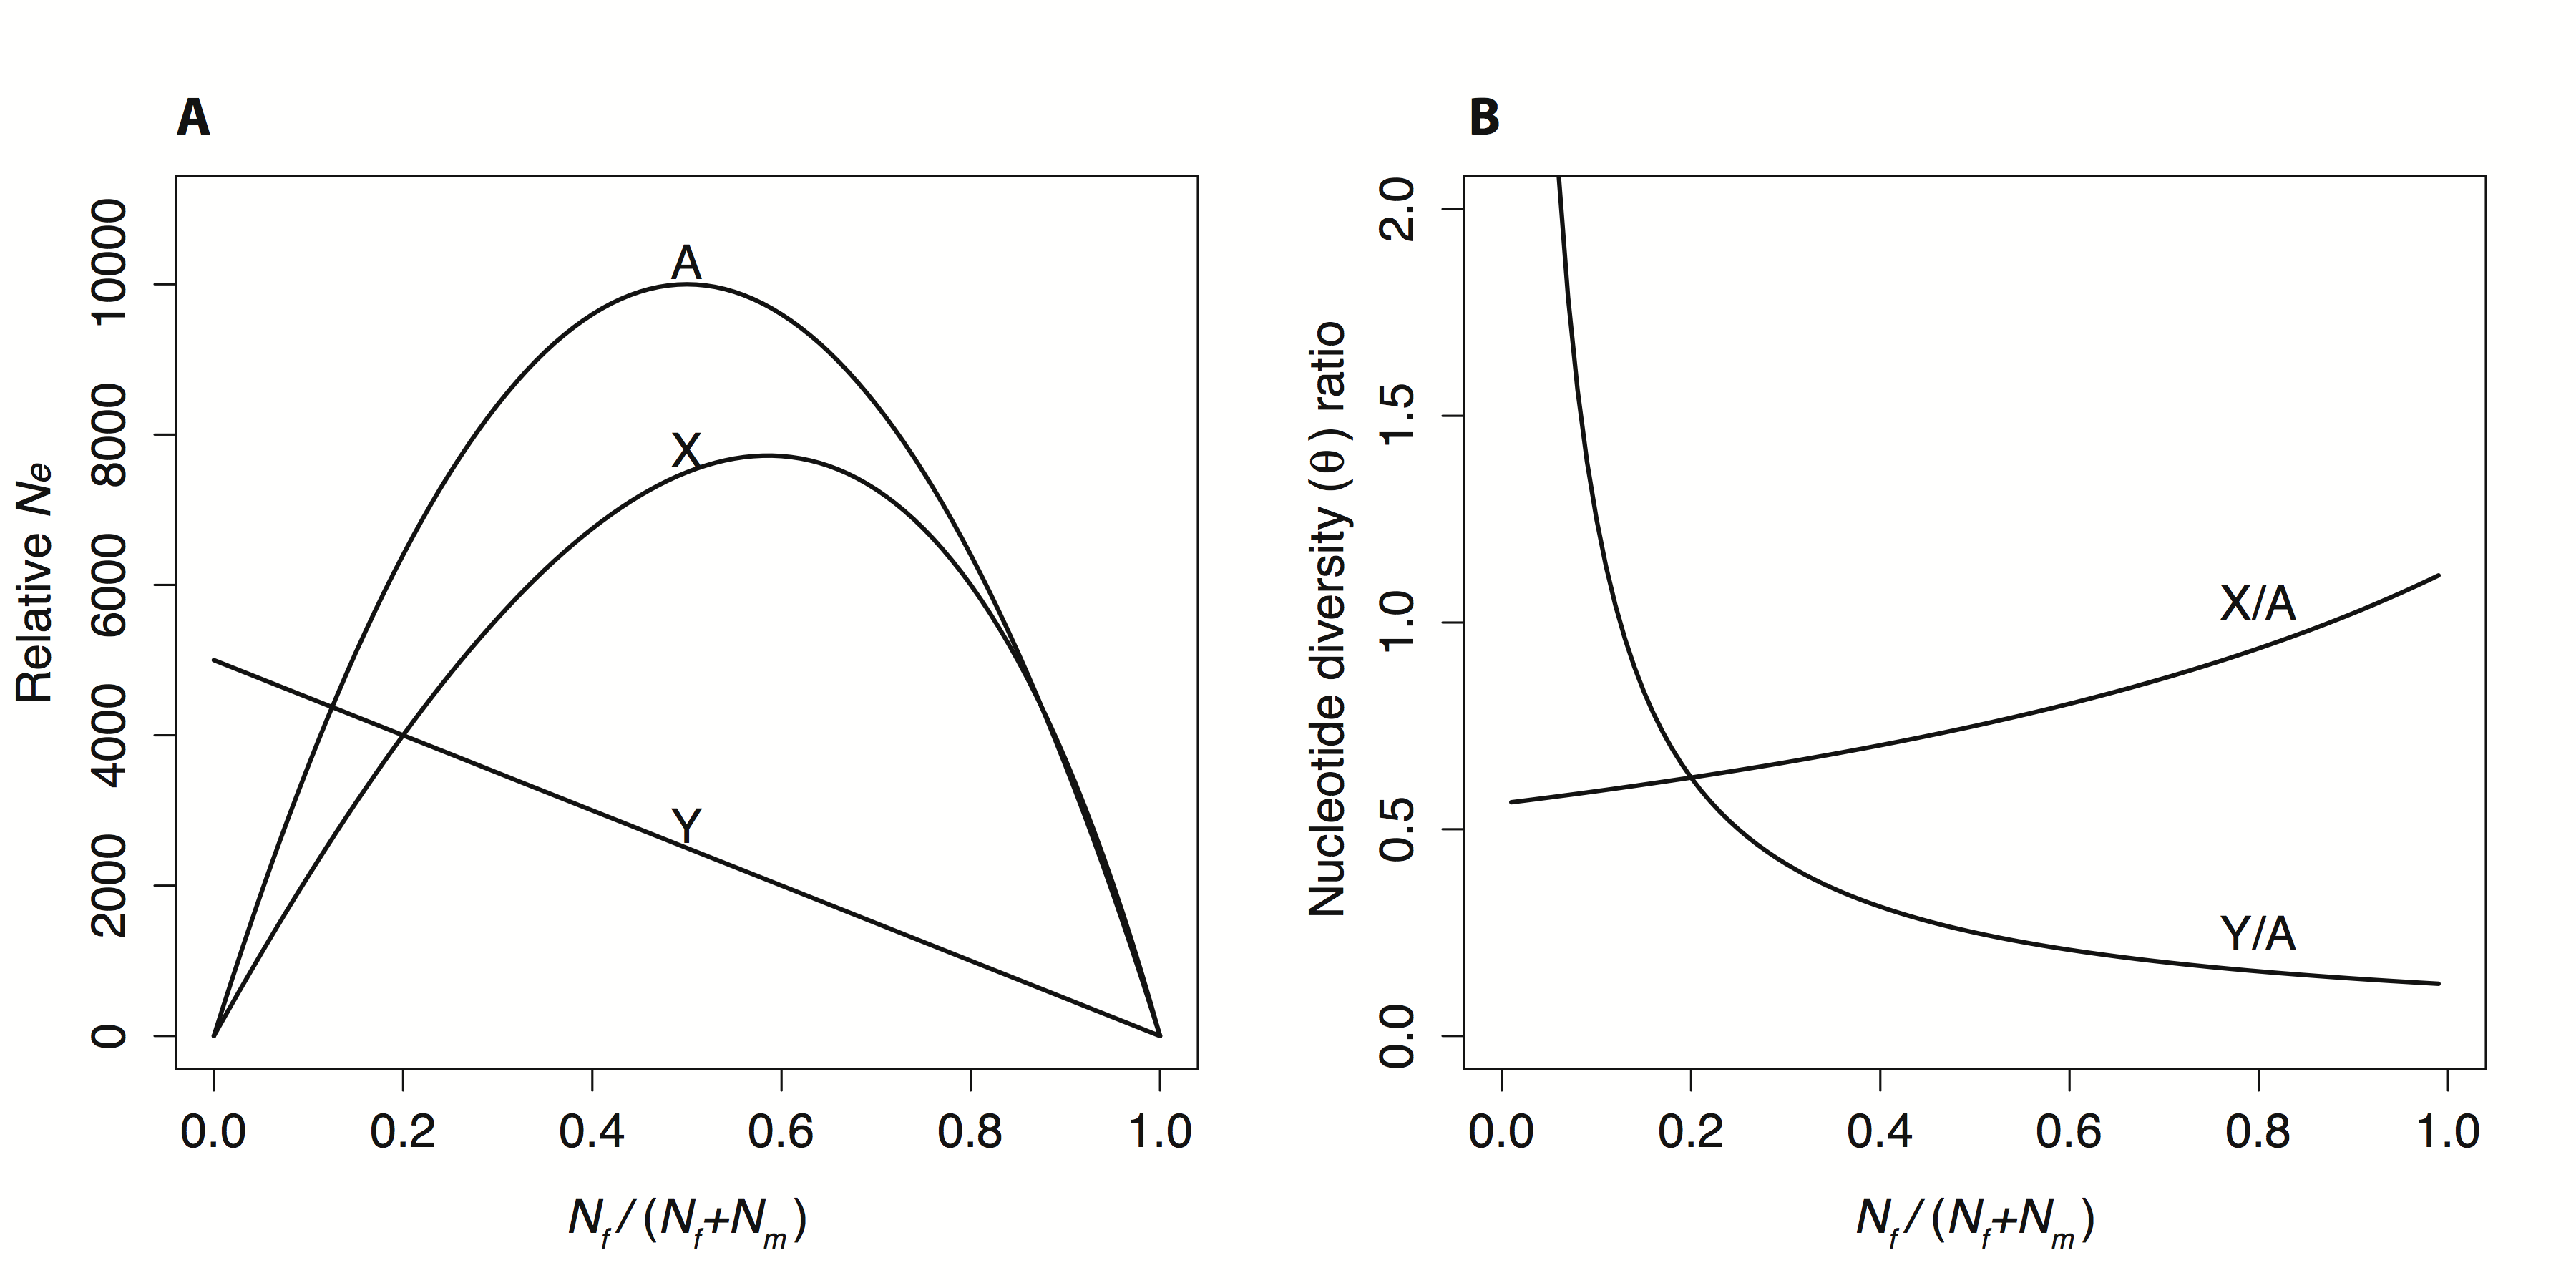
\includegraphics[width=\linewidth]{Figure1.png}
\caption{The relation between relative effective population size and sex ratio bias for genes on autosomes (\textbf{A}) and sex chromosomes (\textbf{B}) (Y chromosome in red). The sex ratio is shown as the proportion of males, $N_{m}/(N_{f}+N_{m})$, where $N_{m}$ and $N_{f}$ are the effective number of breeding males and females, respectively, plotted against $N_{e}/N$, where $N=N_{m}+N_{f}$ and the $N_{e}$ for sex chromosomes and autosomes is given in equations 1-3. Dotted curves show predictions in the standard neutral model, where both males and females produce Poisson-distributed offspring numbers and the chromosomal $N_{e}$'s are given by equations 4-6 \citep{wright1931evolution}. Solid curves correspond to increasing levels of variance in male reproductive success \citep{nomura2002effective} (see Methods). Assuming $\theta=4N_{e}\mu$ and equal neutral mutation rates among genes, the predicted $N_{e}$'s are used to generate null predictions for X/A and Y/A ratios of diversity.
}
\label{fig:spectrum}
\end{figure}

\subsection*{Simulations of positive and purifying selection}
To test whether our observed level of Y-chromosome diversity could be explained by the effects of linked selection, we followed the approach used in \citep{Wilsonsayres2014} and conducted forward-time simulations using the software SFSCODE \citep{hernandez2008flexible} and compared our empirical diversity estimates with those from simulations. This approach was preferred over using analytical predictions primarily because the background selection model over-predicts the reduction in diversity when there are many linked sites under selection \citep{KaiserCharlesworth}, as is expected to be the case for Y chromosomes that lack crossing over.

For purifying selection simulations, we assumed that selection coefficients followed a gamma distribution, and we considered a range of values for the mean selection coefficient against deleterious mutations, $s$, by varying the scale parameter from 0.0001 to 0.1 while keeping the distribution shape parameter constant (see Supporting Information for simulation commands). To make the simulation output comparable to our data, we initialized the simulations with our empirically estimated autosomal $\theta$, adjusted for a sex ratio of $N_{m}/N_{f}=0.4$, and we sampled 8 haploid chromosomes per simulation. Simulated sequences contained 500 kb of linked neutral sequence from which we calculated diversity.

For positive selection with recurrent hitchhiking, we used sfscoder to implement the method of \citep{uricchio2014robust}, and simulated a 500kb (\X) neutral locus that was flanked by 100kb loci on either side that were subject to positive selection. We ran 1000 replicates for each model and calculated the average $\theta_{Y{sim}}$ values and the corresponding Y/A ratios for each model seperately. Finally, we tested the significance of the fit of the simulated diversity to our empirical Y/A ratio (\X new figure) by calculating the proportion of simulation replicates for which $\theta_{{Y}sim}$ was not significantly different from $\theta_{{Y}observed}$, using a two-sided P value. Commands for running the simulations are provided in the Supporting Information.

\section*{Results and Discussion}

\subsection*{Y-chromosome diversity in \textit{R. hastatulus} is very low}
Our analysis revealed that diversity on the \textit{R. hastatulus} Y chromosome is significantly lower than expected under neutrality, with estimates indicating Y/A=0.02, which is 12.5 fold lower than the standard neutral prediction of Y/A = 0.25 (P<0.0001), and 40-fold lower compared to mean diversity on the X chromosome (Table 1). Note that by normalizing X and Y diversity by autosomal diversity, our results indicate that the X-Y difference we observed was not due to an elevation of X chromosome diversity, but rather a Y-specific reduction. Conceivably, such low diversity on the Y could arise from a low mutation rate on the Y chromosome, or a lower mutation rate in males compared to females. However, these possibilities can be rejected because there is no evidence that the number of synonymous mutations in X and Y lineages, estimated by both parsimony and maximum likelihood, are significantly different \citep{hough2014}.

\begin{table}[t!]
\centering
\caption{Estimates of neutral diversity by race on \textit{R. hastatulus} sex chromosomes and autosomes.}
\begin{tabular}{ccccccccc}
\textbf{} & \multicolumn{2}{c}{\textbf{Texas}} & \multicolumn{2}{c}{\textbf{South Carolina}} & \multicolumn{2}{c}{\textbf{Florida}} \\
chromosome & $\theta$ & $\theta/\theta_{A}$ & $\theta$ & $\theta/\theta_{A}$ & $\theta$ & $\theta/\theta_{A}$ \\
\midrule
A & 0.006 & 1 & 0.006 & 1 & 0.005 & 1 \\
X & 0.0047 & 0.85 & 0.002 & 0.33 & 0.0047 & 0.37 \\
Y & $\num{e-4}$ & 0.002 & $\num{e-4}$ & 0.002 & $\num{e-4}$ & 0.002 \\
\addlinespace

\bottomrule
\end{tabular}
\end{table}

Although our sampling of each \textit{R. hastatulus} sub-clade is limited, the discovery of three phylogenetically distinct monophyletic groups is interesting because it suggests the possibility that introgression occurred between the ancestral Texas (XY race) and the derived North Carolina ($XY_{1}Y_{2}$) race, leading to a derived $XY_{1}Y_{2}$ sub-clade. As the North Carolina and Texas races are known to be inter-fertile \citep{smith1964evolving}, we suggest that the SC sub-clade inferred here likely originated through hybridization between a female from the FL clade harboring the X-autosome fusion, and a male from the XY Texas race. Notably, when we pooled the samples from each sub-clade together, the estimated level of Y diversity was significantly higher in the pooled data, highlighting the presence of strong substructure between these groups (Figure S2).

Our results also indicate a significant reduction in X/A diversity in the derived SC and FL sub-clades of the North Carolina race ($X/A_{FL}=0.33$ and $X/A_{SC}=0.37$) compared to the Texas race ($X/A_{TX}=0.85$) (Figure 2). Although not expected, this reduction in diversity may be associated with the recent origin of the $XY_{1}Y_{2}$ sex chromosome system, which is thought to have originated through an X-autosome fusion involving the ancestral 3rd chromosome in the Texas race \citep{smith1964evolving}. Evidence supporting this autosomal origin was recently obtained by \citep{grabowska2015}, who reported that the ancestral third chromosome in the Texas race carries the 5S rDNA locus, which is now found on both the neo-X and the $Y_{2}$ sex chromosomes in the derived North Carolina race. If recent positive selection was involved in driving the evolution of this X-A fusion, which theory suggests can driving the evolution of such fusions \citep{charlesworth1980sex}, then the formerly autosomal segment on the X chromosome in the $XY_{1}Y_{2}$ sub-clades may have experienced a strong selective sweep, resulting in reduced X-linked diversity in the derived $XY_{1}Y_{2}$ sub-clades. It will be important for future work to investigate in more detail the factors driving the establishment of the X-autosome fusion in this species, and how they might impact patterns of X-linked neutral diversity.

In contrast to the X chromosome, however, our data indicate a strong and consistent diversity reduction on the Y chromosome: an approximately 40 fold reduction compared to the mean $\theta_{X}$. We next consider several possible models - neutral and selective - that might explain this reduction.

\subsection*{Female biased sex ratio and high variance in male fitness}

 The occurrence of female-biased sex ratios in this species has been predicted to lower Y diversity due to its effects on reducing male $N_{e}$ and therefore the neutrally expected $N_{e}$ of the Y chromosome (\X ref). This reduction $N_{e}$ on the Y is expected to be further accented if there is high variance in male reproductive success (Figure 1), which is not unusual in annual plants such as \textit{R. hastatulus} that commonly exhibit extensive phenotypic plasticity in plant size and flower production (\X Harper 1977). Moreover, given that male plants in this wind-pollinated species produce large amounts of pollen, and that female flowers are uniovulate, we expected that there is strong competition among males to fertilize females.

 In common with most flowering plants we do not have marker-based estimates of the variance in male reproductive success in \textit{R. hastatulus}. However, by comparing our empirical estimates of diversity to predictions from models that jointly predict the effects on diversity of sex ratio bias and male reproductive variance, we evaluated whether these effects could explain the level of Y/A diversity that we observed (see Methods). Conditioning on estimates of sex ratio bias in \textit{R. hastatulus} that have been estimated, ranging from $N_{m}/(N_{m}+N_{f})=0.4$ to $N_{m}/(N_{m}+N_{f})=0.35$ \citep{pickup2013influence}, the predicted Y/A diversity ratio  is approximately 0.2 (Table1, Figure 3). This is significantly lower than our estimated mean Y/A ratio of 0.02 ($\textit{P}<0.0001$), and remains significant even if we consider an upper bound estimate obtained from our likelihood based estimated of the confidence interval. This suggests that the sex ratio effect alone is insufficient to explain our data under the standard sex ratio model. (\X I think some of this can be written better...)

Assuming that there is extensive variance in male reproductive success (\X), the predicted ratios of Y/A diversity (\X supp) were also significantly higher than our estimates for the empirically estimated sex ratio (\X table) . We also find, however, that purely neutral models in which the sex ratio was highly female-biased (\X), with level of variance in male reproductive success on the order of (\X), predicted a Y/A ratio that could not be rejected (\X). However, because a highly females biased sex ratio is expected to increase the X/A ratio as well, these models simultaneously predicted a range of X/A ratios that were significantly different from what we observed (\X Figure). Thus, our results indicate that the combined effects of sex ratio bias and variance in reproductive success cannot jointly explain our observed levels of X, Y, and autosomal diversity.

\subsection*{Background Selection and Selective Sweeps}

%Although we do not exclude the possibility that positive selection has also reduced Y chromosome variability, our simulations suggest that the reduction in diversity arising from purifying selection is sufficient to explain our observed patters of neutral variation.

%This reduces their Ne, so that they behave as if they were subject to weaker selection than with free recombination, thereby reducing their effects on linked neutral or nearly neutral variants [9].

%hat genetic variability in these regions can be explained by interference among strongly deleterious mutations

%less effective in influencing the behaviour of neighbouring sites as the number of closely linked sites on a chromosome increases.

%For this chromosome, BGS predicts values of the ratio of neutral diversity to the rest of the genome of  0.1% [9], whereas the observed mean value is  6.5%

%The agreement is reasonably good given the uncertainties involved.

%silent site diversity for 22 genes on the D. miranda neo-Y is
%is  1.2% of the value for their homologues on the recombin- ing neo-X chromosome

% Our observed levels of diversity are essentially at that saturation point, highlighting that we are indeed in a realm where there are a large number of sites subject to purifying selection. So I think we can safely say that, with the caveat about parameter uncertainty, the number of sites under selection is likely to be 800kb or more, consistent with ongoing purifying selection driving down diversity on this chromosome
%This reduces their Ne, so that they behave as if they were subject to weaker selection than with free recombination, thereby reducing their effects on linked neutral or nearly neutral variants [9].

%hat genetic variability in these regions can be explained by interference among strongly deleterious mutations

%less effective in influencing the behaviour of neighbouring sites as the number of closely linked sites on a chromosome increases.

%For this chromosome, BGS predicts values of the ratio of neutral diversity to the rest of the genome of  0.1% [9], whereas the observed mean value is  6.5%

%The agreement is reasonably good given the uncertainties involved.

%silent site diversity for 22 genes on the D. miranda neo-Y is
%is  1.2% of the value for their homologues on the recombin- ing neo-X chromosome

% Our observed levels of diversity are essentially at that saturation point, highlighting that we are indeed in a realm where there are a large number of sites subject to purifying selection. So I think we can safely say that, with the caveat about parameter uncertainty, the number of sites under selection is likely to be 800kb or more, consistent with ongoing purifying selection driving down diversity on this chromosome

%-Although we do not exclude the possibility that positive selection has also reduced Y chromosome variability, our simulations suggest that the reduction in diversity arising from purifying selection is sufficient to explain our observed patters of neutral variation. Given the recent origin of \textit{R. hastatulus} sex chromosomes, our results suggest that the low level of sequence diversity commonly observed on ancient Y chromosomes might evolve relatively quickly after sex chromosomes originate, with selection against deleterious mutations playing an important role during the earliest stages of their evolution.\end{abstract}

It is worth noting that our results only apply to the $Y_{1}$ chromosome, as estimates of diversity were calculated for sex-linked genes that were shared between the $XX/XY$ and the $XX/XY_{1}Y_{2}$ sex chromosome systems. Previous work found that both the $Y_{1}$ and the more recently evolved "neo" $Y_{2}$ chromosomes exhibited signs of genetic degeneration, including gene loss, loss of expression, and an accumulation of amino acid-changing mutations \citep{hough2014}, but we cannot say from the present study whether the neo-Y chromosome has also undergone a reduction in diversity. However, the extensive reduction in diversity estimated on the $Y_{1}$ chromosome occurs in each of the three \textit{R. hastatulus} sub-clades (\X Figure 2; Table 1; Figure S2), suggesting that this effect is not population-specific.

\section*{Conclusions}

\section*{Acknowledgments}


\bibliography{bibliography}
\end{document}
